\documentclass[../Languages.tex]{subfiles}

\begin{document}
\usec{R}\label{sec:r}

\cd{R} is a free programming language and software enviornment for statistical
computing and graphics that is supported by the R Foundation for Statistical
Computing. The \cd{R} language is widely used among statisticians and data
miners for developing statistical software and data analysis. Polls, surveys of
dat aminers, and studies of scholarly literature databases show that \cd{R}'s
popularity has increased substantially in recent years.

\cd{R} is a GNU package. The source code for the \cd{R} software environment is
written primarily in \cd{C}, \cd{Fortran}, and \cd{R}. \cd{R} is freely
available under the GNU General Public License, and pre-compiled binary
versions are provided for various operating systems. While \cd{R} has a command
line interface, there are several graphical front-ends available.

\subsection{Influence}\label{sub:influence}

\begin{Figure}
  \centering
  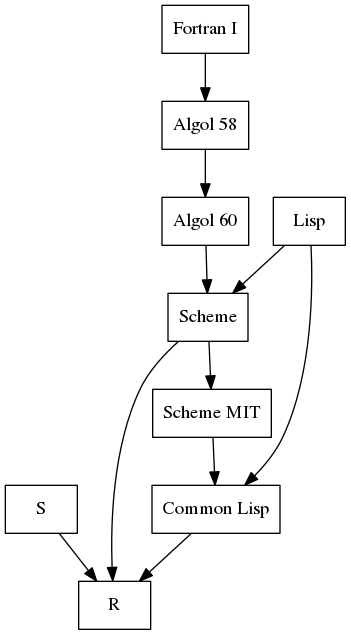
\includegraphics[height=0.5\textheight]{r}
  \captionof{figure}{Inheritance diagram for \cd{R}.}
\end{Figure}

\newpage
\end{document}
